\documentclass[10pt, english]{article}

\title{\textbf{Continuous Active Learning with Systematic Reviews in Medicine}}
\author{
    \fontsize{11}{13}\selectfont 
    Aaron HA Fletcher \\
    \fontsize{10}{11}\selectfont 
     School of Computer Science\\
    \fontsize{10}{11}\selectfont 
    Sheffield\\
    \fontsize{10}{11}\selectfont
    ahafletcher1@sheffield.ac.uk\\
}
\date{}
%%%%%%%%%%%%%%%%%
% import packages %
%%%%%%%%%%%%%%%%%
\usepackage{lipsum}
\usepackage{lmodern} % customize author's fontsize
\usepackage{ragged2e}
\usepackage{adjustbox}
\usepackage{array}
\usepackage{rotating}
\usepackage{array}
\usepackage{setspace}
\usepackage{algorithm}
\usepackage{algpseudocode}
\usepackage{multirow}
\usepackage{booktabs}
\usepackage{makecell}

\usepackage{amsmath}
\usepackage{amssymb}
\onehalfspacing
\def\mystartdate{2022-3-1}%starting date of the calendar
\def\myenddate{2022-4-30}%ending date of the calendar

\usepackage{tikz}
\usetikzlibrary{shapes,arrows,positioning,fit,backgrounds}
\usetikzlibrary{arrows.meta, positioning, calc}

% setting page settings and layout 
% https://texdoc.org/serve/geometry/0
\usepackage[
layout=letterpaper, 
paper=letterpaper, 
portrait, 
head=0.5in,
foot=0.5in,
top=1in, 
bottom=1in, 
left=0.75in, 
right=0.75in
]{geometry}
\usepackage[english]{babel}
\setlength{\columnsep}{0.25in} % space/gap between columns
% \pagenumbering{gobble}  % suppress page number
\usepackage{xurl}
% \usepackage[hyperpageref]{backref}	 %  link to bib citations
\usepackage[runin]{abstract}
\usepackage{tabularx}

\usepackage{hyperref} % it needs to come before biblatex
\hypersetup{
colorlinks=true,
urlcolor=blue,
linkcolor=blue,
citecolor=blue,
pdftitle={@title - @author},
pdfsubject={Systematic Review},
pdfauthor={@author},
pdfkeywords={list; here; your; keywords (key words)}
}
\usepackage[style=numeric-comp,backend=biber,backref=true,sorting=none]{biblatex}
\usepackage{cleveref}

\addbibresource{zot_references.bib}
\usepackage{etoolbox}
\usepackage{csquotes}
\usepackage{indentfirst} % indent section's paragraphs
\def\ni{\noindent} % remove abstract paragraph
\usepackage{custom_commands} % custom commands, including abstract text
\usepackage{subfiles} % best loaded last in the preamble
\usepackage{graphicx} % add images
\usepackage{titlesec}
\usepackage{fancybox} % boxes
\usepackage{soul,color} %highlighter
\usepackage{amsmath}
\usepackage{pdfpages}
\usepackage{tocloft}
\setlength{\cftsecnumwidth}{2.5em}
\usepackage{pdflscape}
\usepackage{fancyhdr}
\pagestyle{fancy}
\fancyhf{}
\fancyfoot[C]{\thepage}
\renewcommand{\headrulewidth}{0pt}
% \titleformat{\section}{\normalfont\large\bfseries}{}{0em}{}
% \titleformat{\subsection}{\normalfont\large\bfseries}{}{0em}{}W
% \titleformat{\subsubsection}{\normalfont\normalsize\bfseries}{}{0em}{}
\begin{document}
\pagenumbering{arabic}
\renewcommand{\abstractname}{} % remove 'Abstract' title
\maketitle % create title and authors
\newpage



\newpage

%%%%%%%%%%%%
% Abstract %
%%%%%%%%%%%%
%% remove spacing from abstract

\setlength{\absleftindent}{0em}

\begin{abstract}
    \abstractText % see custom_commands
\end{abstract}
\newpage
\tableofcontents
\newpage
\newcommand{\lightshadowbox}[1]{%
  \setlength{\fboxsep}{6pt}%
  \setlength{\shadowsize}{1pt}%
  \shadowbox{#1}%
}

\newpage
%%%%%%%%%%%
% Article %
%%%%%%%%%%%
\section{Introduction}

Systematic reviews are a cornerstone for evidence-based medicine, providing rigorous, high-level research syntheses to guide clinical practice and policy. Yet this rigour carries a steep cost: systematic reviews are labour-intensive, often requiring researchers to screen thousands of documents manually. Technology-Assisted Review (TAR) methods, particularly Continuous Active Learning (CAL), promise to alleviate some of this burden. However, many existing approaches still treat documents as isolated entities, overlooking inter-document relationships or disregarding previously recalled documents' contribution to a search goal.

Manual screening, and even many CAL approaches, shallowly represent documents. That is to say, they use only information sourced from the title and abstract despite many more signals being available (inter-document connections), such as citation networks or metadata (e.g., source of publication, authorship, date of publication). These signals, used instinctively by human operators, could steer the selection for screening towards high-value studies. Moreover, the conventional practice of stopping screening relies on a simplistic, binary categorisation of documents as relevant or not, triggering the stop after a fixed ``target recall" threshold is met. This shallow document representation fails to recognise that documents contribute variably to a review's conclusions. While it provides a seemingly objective benchmark, target recall fails to consider the information's utility. Whether the accumulated evidence sufficiently addresses the research question or whether further screening is likely to produce diminishing returns remains unexamined. 

Further research is needed to tackle these shortcomings through a more information-centric and adaptive approach to automating systematic reviews. First, this research will investigate relationship-aware CAL methods that harness inter-document connections to rank and prioritise more intelligently for screening. Second, this research will examine the value of intra-document information, creating utility-driven stopping criteria that shift the focus from static recall targets to the actual value of newly discovered evidence. Rather than screen indiscriminately to meet a blanket recall requirement, the process stops once the reviewed studies collectively offer a robust answer to the research question. By utilising existing inter-document information or aligning the screening endpoint with genuine evidence needs, the resource demands of systematic reviews can be reduced while maintaining quality.

\newpage
\section{Literature Review}

\subsection{Screening Prioritisation}

%What is screening prioritisation
Screening determines whether a document is relevant to the research question. Reviewers performing systematic reviews screen the title and abstract substage by assessing basic document information (i.e, title and abstract) against predefined eligibility criteria. Existing practice usually treats each document as an isolated entity, neglecting supplementary metadata such as citations, co-authors, or citation frequency.  A second, more resource-intensive full-text review follows to confirm inclusion. Because full-text review is time-consuming, many methods have been proposed to automate or semi-automate the title and abstract screening step—often referred to as prioritisation—to reduce the screening burden.

Prioritisation is the process of ranking documents by their likelihood of relevance. Prioritisation puts the documents at the top of the list that should address the systematic review's research question, enabling reviewers to find relevant literature more quickly. In principle, prioritisation can dramatically reduce screening efforts by allowing a screener to stop once they have located most or all of the relevant articles. For example, consider a hypothetical dataset of 20 documents, with 5 of those being relevant. All 20 must be screened without any prioritisation to find the five that matter. If the documents are ranked perfectly in descending order of relevance, the screener could theoretically locate all five relevant documents by examining only the first 5 in the list, reducing total document reviews. 

Technology-Assisted Review (TAR), also known as Computer-Assisted Review or Predictive Coding, is a process that uses machine learning to assist in document screening. Approaches to TAR fall into two categories: (1) those ranking directly with queries (e.g. the query being the title \cite{alharbi_ranking_2017, alharbi_retrieving_2018}, boolean search terms  \cite{alharbi_ranking_2017, alharbi_retrieving_2018, alharbi_ranking_2019}, or review objectives \cite{ferro_qut_2017, scells_integrating_2017}), and (2) those using indirect methods like relevance feedback \cite{alharbi_ranking_2019} or active learning \cite{cormack_technology-assisted_2017, cormack_systems_2019, grossman_technology-assisted_2010, grossman_automatic_2017}. This research focuses on using active learning, which has successfully been used in many areas of information retrieval \cite{cormack_autonomy_2015, cormack_engineering_2016, yu_fast2_2019, yu_finding_2018, miwa_reducing_2014}.

\subsubsection{Active Learning}

% What is active learning
Deep learning models and other classifiers often require large labelled datasets to perform well. In systematic review screening, gathering labels can be slow and expensive, especially at the outset when little is known about relevance. Active learning aims to mitigate this challenge by selecting the most \emph{informative} unlabelled documents for human labelling in iterative cycles.

This iterative process aims to substantially improve model performance while minimising the time and effort required for labelling. A typical active learning workflow selects a batch of unlabelled samples based on their potential to improve the model. These selected samples are then labelled and incorporated into the growing training dataset. The model is subsequently retrained using this expanded dataset, leading to improved model classification and ranking accuracy. The core principle behind active learning is to balance exploring uncertain or ambiguous documents (exploration) and exploiting documents that are likely to be highly relevant (exploitation). This approach enhances the model's ability to rank documents accurately, making the systematic review process more efficient and effective.

Variations of active learning exist, such as membership query synthesis \cite{angluin_queries_1988}, stream-based selective \cite{akinseloyin_novel_2024} and pool-based sampling \cite{lewis_sequential_1994}. 
Pool-based sampling best suits title and abstract screening because the unlabelled document set is known in advance. Figure \ref{fig:pool_based_query} illustrates this workflow. Mainstream prioritisation approaches largely model documents based on their text alone, such as bag-of-words or embeddings of titles and abstracts \cite{diao_lexical_2021}. Conventional active learning algorithms do not incorporate inter-document relationships; they rely on textual features or basic metadata to measure uncertainty and relevance. This can overlook important ``network-level" cues (e.g., shared references, reciprocal citations, co-authorship clusters) that could guide the active learning process toward the most pertinent articles faster.


\begin{figure}
\centering
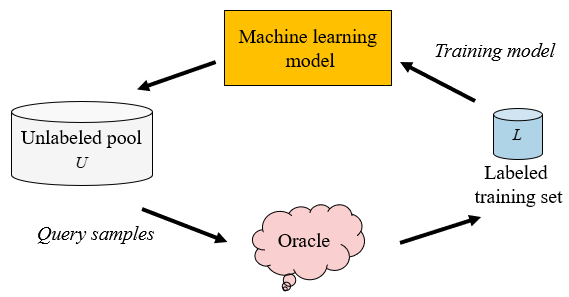
\includegraphics[width=0.5\linewidth]{images/pool_based_strategy.png}
\caption{Overview of a pool-based query strategy for active learning, replicated\cite{ren_survey_2021}}.
\label{fig:pool_based_query}
\end{figure}

% Active Learning Notation 

The active learning process can be formally described as follows:

\begin{enumerate}
    \item A sampling policy ($\pi$) intelligently selects the most informative samples ($\mathbf{T}_{C,i}$) from an unlabelled dataset ($\mathbf{T}_{U,i}$).
    \item These samples are passed to an oracle ($O$) for labelling.
    \item The labelled samples are added to a growing known dataset ($\mathbf{T}_{K,i}$).
    \item A classifier is trained on this labelled dataset.
    \item The classifier ranks the remaining unlabelled samples in ($\mathbf{T}_{U,i}$), often based on the classifier's uncertainty or expected model improvement.
    \item This iterative process repeats, intending to improve the classifier's performance with each labelling round until a predefined stopping criterion is met.
\end{enumerate}

The oracle within systematic reviews denotes a human-verified label resulting from screening potential research for inclusion within the systematic review within the title and abstract screening stage. More concretely, $O$ can be considered a function $O(x) = y$ where $x$ is a document representation (i.e. if a human was reviewing a title and abstract or a representation of the title and abstract for automated approaches), and $y$ is the assigned category (included or excluded). In active learning research, in contrast to research in systematic reviews, it is assumed that for each $x$, $O$ provides a single judgement ($y$), which is always correct.


\begin{table*}[t]
    \centering
    \footnotesize

    \begin{tabular}{|c|c|>{\raggedright\arraybackslash}p{11cm}|}
        \hline
        \textbf{Notation}    & \textbf{Explanation}                            & \textbf{Notes}                                                                                \\
        \hline
        \(\textbf{T}\)       & Total dataset                                   & e.g. Research gathered after Identification phase of the selection process.                   \\
        \hline
        \(i\)                & Iteration                                       & A single cycle within the active learning process.                                            \\
        \hline
        \(\textbf{T}_{K,i}\) & Known datapoints per iteration                  & e.g. research that has been screened by a reviewer                                            \\
        \hline
        \(\textbf{T}_{U,i}\) & Unknown datapoints per iteration                & e.g. research that has not been screened by a reviewer                                        \\
        \hline
        \(\textbf{T}_{C,i}\) & A subset of \(\textbf{T}_{U,i}\) to be labelled & chosen by a policy, datapoints to be screened by a reviewer.                                  \\
        \hline
        $\pi$                & Policy                                          & How \(\textbf{T}_{U,i}\) is selected, e.g. uncertainty, random, certainty, diversity sampling \\
        \hline
        O                    & Oracle                                          & Often a domain expert, who assigns labels to unscreened research.                             \\
        \hline
        \(T_R\)              & Total Relevant Documents                        & All research that should be included in a systematic review.                                  \\
        \hline
        \(T_{IR}\)           & Total Irrelevant Documents                      & All research that should not be included in a systematic review.                              \\
        \hline
    \end{tabular}
    \caption{Notation used for active learning within this review}
    \label{tab:notation}
\end{table*}


% How AL doesn't address systematic review issues

While active learning offers advantages, its direct application to systematic reviews has limitations:

\begin{itemize}
    \item \textbf{Delayed Incorporation of Early Information:} Waiting until a minimum number of documents has been assessed before training the model means valuable information gathered in the early phases is not incorporated into the ranking process.
    \item \textbf{Delayed Search Phase:} The actual search and screening process is delayed until sufficient relevant studies are present in the document collection.
    \item \textbf{Minimum Number of Relevant Studies Required:} A minimum number of relevant studies is often required in the initial document collection. This is usually impractical in the early stages of a systematic review.
\end{itemize}

To truly minimise screening effort, a scenario is needed where minimal expert screening is performed on documents returned from the identification phase, and the model can safely extrapolate that screening to a larger pool.

These disadvantages lead to diversifying TAR approaches. The different TAR approaches have been outlined in Table \ref{tab:differences_in_tar} and can be categorised as follows: Simple passive learning (SPL) \cite{cohen_reducing_2006}, where a ``seed set" of human-labelled documents from $T$ creates the labelled set $T_{K,i}$ used to train a classifier. This classifier then labels $T_{U, i}$ without further learning. Simple Active Learning (SAL), where a ``seed set" of human-labelled documents from $T$ creates the labelled set $T_{K,i}$ is used to train a classifier. This classifier then labels $T_{U, i}$, which is ordered by relevance, and then the most uncertain document labels are revealed. The model is retrained after each batch of newly labelled documents, improving its accuracy. The continuous active learning (CAL) process is similar to SAL; the model is updated continuously, in real-time or near real-time, as human reviewers label documents. There are no discrete rounds; learning is ongoing. The system may still prioritise documents for review based on uncertainty or other strategies, but it can also adapt to reviewer behaviour and potentially re-rank documents on the fly. Cormack et al. \cite{cormack_autonomy_2015} argue that CAL better aligns with systematic review workflows because the goal is to unearth all relevant documents quickly (i.e. exploitation) rather than just optimising model accuracy per see (i.e. balancing exploitation \emph{and} exploration). Nonetheless, as the subsequent research will show, CAL approaches have traditionally treated each document individually rather than utilising the relational structure in the corpus.


\begin{table*}[t]

    \centering
    \footnotesize
    \begin{tabular}{|c|c|c|c|}
        \hline
        \textbf{Feature} & \textbf{Simple Passive Learning} & \textbf{Simple Active Learning} & \textbf{Continuous Active Learning} \\
        \hline
        Learning & One-time, from initial set  & Iterative, in batches  & Continous, real-time \\
        \hline
        Model Updates & None after initial training & After each batch & After each labelled document \\
        \hline
        Reviewer Interaction & None after initial set & Periodic (batch-wise) & Continuous \\
        \hline
        Adaptability & Static  & Moderate & High \\
        \hline
        Prioritisation & Based on initial model & Adapts per batch & Adapts continuously \\
        \hline
    \end{tabular}
    \caption{The key differences between the different forms of active learning within TAR.}
    \label{tab:differences_in_tar}
\end{table*}

\subsubsection{Metadata usage in screening}

% Clarify what is meant by metadata, and where we can find it!
Within this research, metadata refers to the structured or semi-structured information accompanying a publication beyond its raw text—such as author affiliations, publication dates, co-author relationships, journal or conference venues, keywords (including MeSH terms), and other bibliographic details. This metadata is abundant, freely available, and already computed. OpenAlex\footnote{https://www.openalex.org}, for example, is an open-sourced API that covers a large proportion of the literature, providing extensive metadata.

Inter-document relationship refers to citation network analysis, which can be performed using this metadata. So, for example, if a paper cites another, this document is said to be related. Analysis of inter-document relationships and metadata is something that searchers instinctively do when screening documents. To illustrate, if a searcher finds a foundational relevant document, such as Cormack's work on Auto TAR, their other work is likely related to that topic. If a searcher is searching for research on COVID-19, publications before 2019 are not likely to be related. 

The manual approach to title and abstract screening reviews all documents within the total document pool, so inter-document relationships offer little benefit. Interestingly, Backward citation searching (BCS) and Forward citation searching (FCS) are used in the Cochrane approach in the preceding stage, ``identification" that forms the pool~\cite{briscoe_conduct_2020, noauthor_mecir_nodate}. Once the pool of candidate articles is set, the screening phase—where documents are prioritised or ranked—almost always relies solely on each document’s title/abstract, ignoring citation or co-authorship signals that might refine relevance scores. This standard approach—extracting only an article’s abstract and minimal bibliographic fields—overlooks valuable signals embedded in established citation networks, co-author clusters, and publication venues.

Despite the substantial research on automating systematic review screening, most approaches rely almost exclusively on a document’s title and abstract (rarely supplemented with keywords or MeSH terms). A recent scoping review of PubMed-indexed studies on systematic review automation (covering 123 articles) demonstrates this gap clearly: Tóth et al. found that the great majority of record-screening automation tools (broadly utilising SPL, CAL or SAL approaches) used either bag-of-words or TF-IDF representations of the title and abstract text, with only a small proportion incorporating additional metadata such as publication date or author information \cite{toth_automation_2024}. Indeed, a typical pipeline in these tools converts the abstract into a vector of token counts or embeddings and then applies a machine learning classifier or an active learning framework to predict relevance. While a handful of studies appended ``bibliographic details” or ``MeSH terms,” Tóth et al. note that these uses of metadata are inconsistent, rarely extend beyond indexing keywords and do not systematically exploit richer inter-document relationships (e.g., citation networks, co-authorship, or shared references). The author has not identified studies that incorporate metadata into CAL in a structured way. 

Addressing this gap represents both a challenge and a major opportunity. Incorporating structured metadata into CAL prioritisation pipelines could improve recall by surfacing relevant clusters of connected documents earlier. Simultaneously, it may reduce screening workloads by deprioritising documents in low-yield regions of the citation or co-authorship graph. Thus, research into CAL here is viewed through the lens of how they represent documents and if they consider inter-document relationships.  

\subsubsection{Continuous Active Learning for Systematic Reviews}

Recall targets in systematic reviews differ from other domains (e.g.\ e-discovery in law or social-media sentiment analysis) by demanding near-complete recall to ensure no critical study is missed. In medical research, overlooking even a single relevant article can critically affect the interpretation of evidence. Despite this demanding requirement, CAL has shown promise for reducing systematic review screening workloads by up to 77\%~\cite{van_der_vet_propagation_2016}. Nonetheless, current CAL approaches for systematic reviews still largely treat documents as stand-alone entities, relying on shallow representations (e.g.\ bag-of-words or simple neural embeddings) and giving limited attention to inter-document relationships (e.g.\ shared citations or authorship).

To understand the evolution of CAL methods and identify opportunities for incorporating relational signals, the author categorises existing approaches based on how they represent documents (i.e., feature-based vs \ encoder-based vs \ decoder-based). A Feature-based approach is where the title and abstract are transformed into numerical vectors representing features like word presence or importance (e.g., TF-IDF); an Encoder-based approach, where models like BERT capture semantic relationships between words in the title and abstract using a masked self-attention mechanism; and a Decoder-based approach is where generative models like GPT predict the probability distribution of the next word in a sequence, leveraging unidirectional context. Such a taxonomy helps illustrate the progression from methods relying on simple lexical features to those capturing increasingly complex semantic relationships and ultimately highlights the potential for incorporating relational information.

\paragraph{Feature-based Approaches: }

These methods, while foundational, represent documents as isolated entities. They typically transform document text (title and abstract) into numerical vectors, where each dimension represents a specific feature, such as the frequency of a term (e.g., TF-IDF). A common characteristic of these methods is their treatment of documents as relatively independent entities, focusing primarily on word-level importance without explicitly modelling the inter-document relationship.

Cormack et al.~\cite{cormack_evaluation_2014} introduced a foundational feature-based CAL approach using a Support Vector Machine (SVM) classifier. Their method trained a Support Vector Machine (SVM) classifier on an initial set of documents identified through keyword seeding. While this work demonstrated the superiority of CAL over traditional screening methods in an e-discovery context, it presented limitations when applied to the specific requirements of systematic reviews. Notably, the use of a large, fixed batch size (1,000 documents) and a focus on achieving recall@75\% are not well-aligned with the need for near-total recall and adaptive learning in medical literature reviews. Moreover, no leveraging of relational structure inherent in medical literature was used.

While subsequent research, like Auto TAR~\cite{cormack_autonomy_2015}, explored refinements such as alternative term weighting (e.g., Cornell ltc) and batch size optimisation, these methods still primarily focus on word-level importance within individual documents; Auto TAR approach is outlined in Figure~\ref{fig:autotar_process}. Auto~TAR differed from the foundational system by using a single seed document (instead of 1,000) and incrementally increasing by approximately 10\% each iteration, rounded up, demonstrating improved performance and better alignment with systematic review screening. It used Cornell ltc term weighting \cite{salton_smart_1965} to represent documents. Auto~TAR has remained a de facto baseline in many CAL studies, sometimes called the ``base model implementation" (BMI).

\begin{figure}
    \centering
    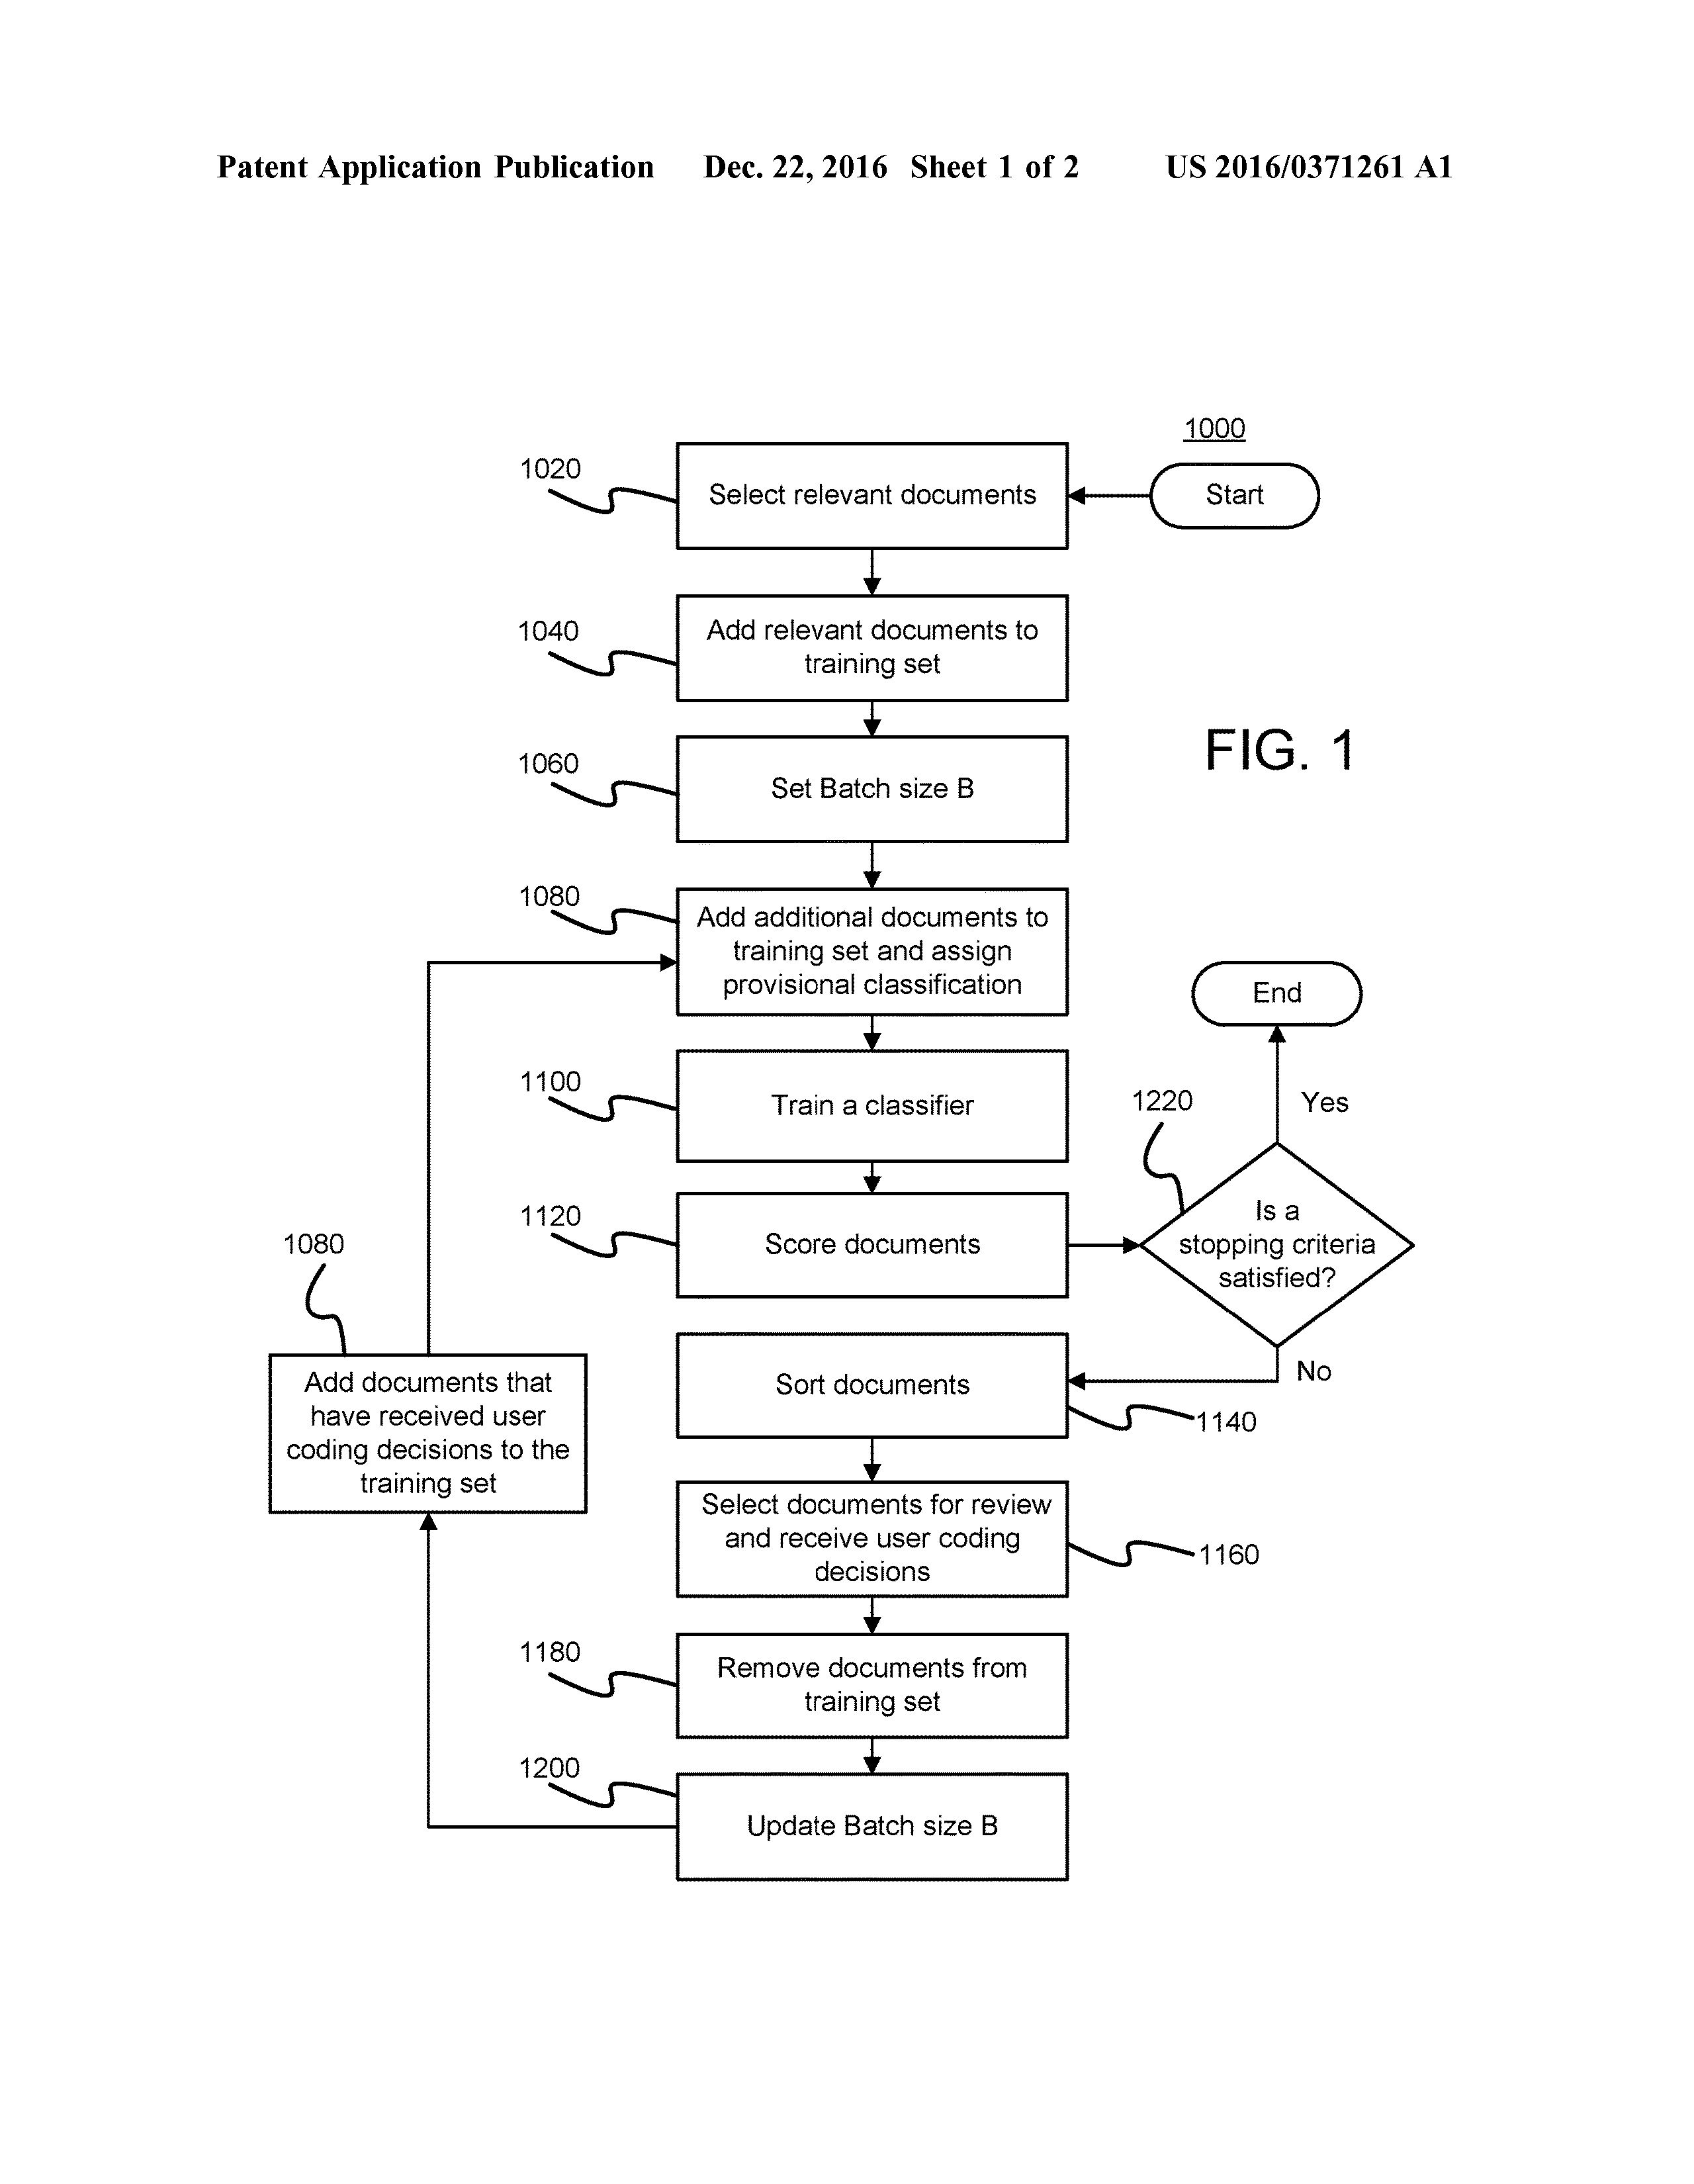
\includegraphics[width=1\linewidth]{images/autotar.jpg}
    \caption{Auto TAR outline, as documented within the patient filing by Cormack et al. \cite{cormack_systems_2016}}.
    \label{fig:autotar_process}
\end{figure}

More recent work has examined hyperparameter choices within feature-based CAL pipelines. Ferdinands et al.~\cite{ferdinands_performance_2023} simulated human reviewers screening six labelled systematic reviews, comparing four classifiers (Naive Bayes, Logistic Regression, SVM, Random Forest) under two document representations (TF-IDF vs.\ doc2vec). The results indicated that Naive Bayes with TF-IDF features reduced the average time to discovery. However, none of these systems integrated metadata or inter-document relationships.

% Approach looking at sentence-level classification vs document-level
Incorporating more information in the screening stage is a step towards richer representations, but they fail to leverage inter-document relationships fully. Although standard feature-based CAL often relies on the title and abstract alone, Zhang et al.~\cite{zhang_evaluating_2020} showed that using isolated representative sentences (via a TF-IDF-based approach) could achieve comparable accuracy and higher efficiency than the BMI. These experiments did not use medical domain datasets and utilised full-text documents, but the study hints at the potential gains from more nuanced feature engineering. Other work has examined MeSH keywords \cite{miwa_reducing_2014} and Latent Dirichlet Allocation (LDA) \cite{hashimoto_topic_2016, miwa_reducing_2014} to enrich feature sets and showed promising performance improvements. This work demonstrates the potential for exploring alternative, superior representations beyond titles and abstracts.

% Incorporating semi-supervision via label propagation
Through incorporating citation proximity, Kontonatsios et al.'s work on label propagation highlights the potential of relational information ~\cite{kontonatsios_semi-supervised_2017}. It introduced a label-propagation method in which a small batch of human-labelled abstracts assign provisional labels (in TF-IDF or spectral-embedded space) to nearby unlabelled citations. These pseudo-labelled documents augment the training pool, accelerating the active learning process. The approach surfaced relevant papers significantly earlier than purely supervised strategies — reinforcing the notion of leveraging unlabelled data and relational signals (e.g.\ local neighbourhoods in feature space) to increase recall. Kontonatsios et al.’s results enhanced recall without imposing an additional annotation burden. This motivates further exploration of semi-supervised paradigms in future CAL systems, especially with advanced document embeddings and network-based relationships.

% Summary of feature-based CAL
In summary, feature-based CAL has proven robust and is a strong baseline.  However, these methods view documents as isolated or rely only on limited textual features (TF, TF-IDF, or keywords). \emph{They do not exploit deeper semantic embeddings or intricate inter-document relationships}, leaving a clear research gap. Though these feature-based techniques paved the way for CAL in systematic reviews, they typically ignore nuanced contextual signals among documents. This omission impedes refined strategies for prioritising and terminating screening. The next section explores whether encoder-based methods offer a deeper representation — and possibly an avenue to more context-aware CAL.

\paragraph{Encoder-based Approaches: }
% Encoder based approaches

Encoder-based models like BERT capture deeper semantic relationships within documents but typically do not explicitly model relationships between documents. Self-attention mechanisms have revolutionised the field of Natural Language Processing, significantly improving performance across a wide range of tasks \cite{vaswani_attention_2023}. However, CAL processes did not fully leverage these advancements initially. The major contribution of self-attention lies in its ability to generate context-dependent text representations, allowing for a more nuanced understanding of text compared to earlier feature-based methods. This capability enables self-attention models to capture subtle semantic relationships and long-range dependencies often missed by traditional approaches like TF-IDF, which were previously dominant in TAR.

Encoder-based models, such as BERT, PubMedBERT and BiolinkBERT, achieve high performance on classification tasks through a two-step process of pre-training (where a model has initially trained large corpora of text to develop a general understanding of language and the specific domain) and fine-tuning (where a pre-trained model is further trained on small,task-specific datasets to adapt it for the particular task). 

Initial work like CALBERT explored incorporating encoder-based models but did not demonstrate superiority \cite{sadri_continuous_2022}. CALBERT ranks a pool of documents using a logistic-regression-based–based CAL model, then refines the top $k$ documents with a BERT-based reranker. Each selected document (title + abstract) is truncated to 512 tokens, converted into an embedding via BERT's CLS token, and passed through a fully connected layer to produce a relevance score. After presenting the highest-scoring document for user feedback, CALBERT is fine-tuned on this new relevance information, and the underlying CAL model is also retrained. However, despite the appeal of using transformers for feature-rich document representations, CALBERT often underperforms the simpler BMI. Variations such as appending the query text (monoBERT) or continuously fine-tuning BERT did not yield consistent gains in a high-recall setting. 

Further research explored pre-training strategies that hindered encoder-based CAL. Yang et al. \cite{yang_goldilocks_2022} fine-tuned a pre-trained BERT on an unlabelled corpus (testing 0-10 epochs) before applying it to CAL. They iteratively sampled 200 documents, labelled them, and fine-tuned BERT for 20 epochs, using the previous iteration's model as the starting point. They found that five epochs of initial fine-tuning yielded performance comparable to TF-IDF and logistic regression on an in-domain dataset but significantly worse on an out-of-domain dataset. This could be attributed to ``catastrophic forgetting" \cite{xu_forget_2020}, where excessive fine-tuning on the task corpus causes the model to lose general knowledge from pre-training. However, Mao's subsequent research suggested that the optimal pre-training epoch (coined ``goldilocks" epoch) CAL was not universal, especially in medical datasets \cite{mao_reproducibility_2024}. Mao's most performant model was not fine-tuned, but rather a model that uses a graph-based approach to pretrain, ${\text{BiolinkBERT}}_{\text{base}}$.

BioLinkBERT incorporates citation links during pre-training and represents a significant step towards leveraging relational information. It is the most performant encoder model on the CLEF dataset in a CAL setting to date. The LinkBERT approach to pre-training models was to view a pertaining corpus as a graph of documents, with each document being a vertex and hyperlinks forming edges between documents \cite{yasunaga_linkbert_2022}. These linked documents were then placed within the same context, different from that of BERT random document allocation, in which no linkage between documents within a context window is required. LinkBERT differs from curriculum learning, where a model is provided with examples of increasing difficulty, as the context windows' documents are not ordered by difficulty. A domain-specific variant of LinkBERT, BioLinkBERT\footnote{https://huggingface.co/michiyasunaga/BioLinkBERT-base}, was created, which was pre-trained only on PubMed articles, with linkage of documents being determined through citations of that research. Models were then trained using standard masked language modelling and next-sentence prediction. The performance of a base model (100M parameters) and a large model (340M parameters) was compared to PubMedBERT\footnote{https://huggingface.co/microsoft/BiomedNLP-BiomedBERT-base-uncased-abstract-fulltext} in BLURB~\cite{gu_domain-specific_2021}, MedQA-USMLE~\cite{jin_what_2021}, and MMLU-professional medicine (medical-specific downstream benchmark tasks)~\cite{hendrycks_measuring_2021}. ${\text{BiolinkBERT}}_{\text{large}}$ achieved state-of-the-art on all reported benchmarks, with an improvement in the BLURB score of 3.2\% above PubMedBERT.

Sparse encoder approaches like SPLADE for CAL have recently been explored outside the medical domain. It leverages a masked language modelling head to expand each token in a document based on contextual cues from the surrounding text. Rather than extracting a single [CLS] embedding, SPLADE predicts a full vocabulary distribution for each token and aggregates these token-level distributions (via max pooling and sparsity regularisation) to form a sparse document representation. This technique preserves many advantages of bag-of-words approaches (e.g., interpretability, efficiency) while injecting knowledge gleaned from large-scale language model pre-training.

Yang et al. found that replacing TF–IDF or BM25 features with SPLADE-based sparse vectors yields a 10–20\% cost reduction \cite{yang_contextualization_2024}. Crucially, these gains arise because the model can capture synonyms, paraphrases, or other subtle relationships that purely lexical methods miss—accelerating the discovery of relevant studies. This highlights how richer, context-aware document representations enhance the effectiveness of CAL, especially under the demanding requirement of near-total recall. The efficacy of medical pre-trained models using SPLADE on medical TAR datasets has not been explored.

% https://arxiv.org/pdf/2407.00635 - dense retrieval - is query based

\paragraph{Decoder-based Approaches: }
Decoder-based approaches, such as LLM+CAL have been outlined and included in this literature review for completeness, as decoder-based work is highly tpoical. In the typical decoder-based approach, a prompt (with or without explanatory examples) is sent to a model, which generates text/tokens in response. Where BERT encodes a passage as a hidden representation, GPT-based models generate text from a unidirectional context.

Decoder-based CAL approaches used prompt engineering with a chain-of-thought approach. Bron et al. proposed a novel method, LLM+CAL, that leverages the capabilities of decoder-based LLMs to enhance the screening process in systematic literature reviews~\cite{bron_combining_2024}. This contrasts significantly with the encoder-based methods discussed previously, which primarily focus on generating contextualised representations for ranking. Bron et al.'s approach focuses on developing more fine-grained and explainable classifications by prompting the LLM to evaluate each document against individual inclusion criteria specified in the review protocol. Instead of a single binary inclusion/exclusion decision, the LLM provides a structured response with reasoning and cited evidence (rationales) for each criterion. This study was, however, only run on a single dataset (Post-traumatic stress disorder systematic review), and the generalisability of this approach is yet established. This criterion-level classification is a unique aspect of their work. It offers potential advantages in integrating LLMs to generate 'synthetic' metadata about a document, which can be combined with a document representation. While this approach demonstrates the power of LLMs, they still largely focus on individual documents.

Work on prompt selection in decoder-based approaches has demonstrated that active learning can be used to select better representative examples for shot prompting.  Baseline, zero-shot prompting not in an active learning process showed good results on a medical dataset, comparable to decoder BioBERT approaches~\cite{wang_zero-shot_2024}. Few-shot prompting also resulted in better performance \cite{margatina_importance_2022} in combination with active learning. It showed that using active learning to identify and choose the most representative examples significantly improved few-shot prompt performance on downstream tasks. This suggests that strategically combining active learning with prompt engineering could enhance the effectiveness of decoder-based models in TAR, even with limited labelled data. While this approach demonstrates the power of LLMs, they still largely focus on individual documents, analyzing them against inclusion criteria. Even active learning for prompt selection, while improving inter-document representation for prompting, does not yet address the crucial need to model inter-document relationships.  This suggests that while decoder-based methods hold promise, further research is needed to incorporate relational information into their frameworks explicitly. 

While decoder-based approaches might be able to produce rationales or explanations, their ability to handle large-corpus level inter-document relationships is limited by their context window size, which restricts the number of documents and relationships they can represent in a single context.

\paragraph{Conclusion: }
The reviewed literature consistently demonstrates the benefit of moving beyond shallow text representations. However, even the most advanced encoder- and decoder-based methods do not explicitly utilise the rich inter-document relationships present in medical research.  Incorporating these relationships is crucial for improving CAL in systematic reviews. Graph Neural Networks offer a natural way to represent and reason about these relationships, making them a promising avenue for future research.


\printbibliography
\end{document}

